% A0: https://de.onlineprinters.ch 86,10 x 120,90 cm with endformat of 84,10 x 118,90 cm
\documentclass[portrait,final,paperwidth=84.10cm, paperheight=118.90cm,showframe fontscale=0.277,margin=1.5cm]{baposter}
\usepackage{relsize}
\usepackage{graphicx}
\usepackage[utf8]{inputenc}
\usepackage{enumitem}
\usepackage[style=ieee, backend=bibtex]{biblatex}
\addbibresource{papers.bib}

% Package list
\usepackage{amsmath,amsthm,amssymb,latexsym} 
\usepackage{xcolor}
\usepackage{hyperref}
\hypersetup{colorlinks,
	citecolor=black,
	filecolor=black,
	linkcolor=black,
	urlcolor=lightgray
}
\sloppy

\RequirePackage{wrapfig}


% Document
\begin{document}
%%%%%%%%%%%%%%%%%%%%%%%%%%%%%%%%%%%%%%%%%%%%%%%%%%%%%%%%%%%%%%%%%%%%%%%%%%%%%%
%%% Here starts the poster
%%%---------------------------------------------------------------------------
%%% Format it to your taste with the options
%%%%%%%%%%%%%%%%%%%%%%%%%%%%%%%%%%%%%%%%%%%%%%%%%%%%%%%%%%%%%%%%%%%%%%%%%%%%%%
% Define some colors
\definecolor{mintish}{RGB}{165,215,210} % Defines the color used for the background
\definecolor{anthrazit}{RGB}{45,55,60}   % Defines the color used for content header

\hyphenation{resolution occlusions}
%%
\begin{poster}%
	% Poster Options
	{
		% Show grid to help with alignment
		grid=false,
		% Column spacing
		colspacing=1.5em,
		columns=4,
		% Color style
		bgColorOne=mintish,
		bgColorTwo=red,
		titleColor=anthrazit,
		footerColor=anthrazit,
%		bgColorTitle=white,
		borderColor=green,
		headerColorOne=anthrazit,
		headerColorTwo=anthrazit,
		headerFontColor=white,
		boxColorOne=white,
		boxColorTwo=white,
		% Format of textbox
		textborder=none,
		% Format of text header
		eyecatcher=false,
		headerborder=none,
		headerheight=0.10\textheight,
		textfont=professionalfonts, %An example of changing the text font
		headershape=rectangle, % rectangle, rounded, smallrounded, roundedleft, roundedright
		headershade=plain, % shade-lr, shade-tb, shade-tb-inverse, plain
		headerfont=\large\bf\textsc, %Sans Serif
		textfont={\setlength{\parindent}{1.5em}},
		boxshade=plain,
		background=plain, % shadeLR, shadeTB, user, none
		titlebackground=plain, % plain, none
		footerbackground=plain, % plain, none
		linewidth=2pt,
		boxpadding=0.8em,
	}
	% Eye Catcher
	{
		
\includegraphics[height=4.0em]{logo/UniBas_Logo_EN_Weiss_Trans_RGB_55}
	} 
	% Title
	{\textcolor{white}{\Huge\bf\textsc{A very very very long multi-line \\paper title}}\vspace{0.2em}}
	% Authors
	{\textcolor{white}{\normalsize{
				\hspace{-0.2em}\textbf{\underline{Author 1}}, Author 2 and Author 3\\
				Department of Mathematics and Computer Science, University of Basel
			%	\{dennis.madsen, thomas.vetter, marcel.luethi\}@unibas.ch
			}
		}
	}
	% University logo
	{% The makebox allows the title to flow into the logo, this is a hack because of the L shaped logo.
			
\includegraphics[height=6.0em]{logo/UniBas_Logo_EN_Weiss_Trans_RGB_55}
	}
	% Footer
	{
		{\textcolor{lightgray}{\normalsize{\bf{
						\noindent \url{gravis.dmi.unibas.ch}\hfill \url{www.brian-amberg.de/uni/poster}\hfill \href{mailto:someone@unibas.ch}{someone@unibas.ch} 
					}
				}
			}
		}
	}
	
	%%%%%%%%%%%%%%%%%%%%%%%%%%%%%%%%%%%%%%%%%%%%%%%%%%%%%%%%%%%%%%%%%%%%%%%%%%%%%%
	%%% Now define the boxes that make up the poster
	%%%---------------------------------------------------------------------------
	%%% Each box has a name and can be placed absolutely or relatively.
	%%% The only inconvenience is that you can only specify a relative position 
	%%% towards an already declared box. So if you have a box attached to the 
	%%% bottom, one to the top and a third one which should be in between, you 
	%%% have to specify the top and bottom boxes before you specify the middle 
	%%% box.
	%%%%%%%%%%%%%%%%%%%%%%%%%%%%%%%%%%%%%%%%%%%%%%%%%%%%%%%%%%%%%%%%%%%%%%%%%%%%%%

	%%%%%%%%%%%%%%%%%%%%%%%%%%%%%%%%%%%%%%%%%%%%%%%%%%%%%%%%%%%%%%%%%%%%%%%%%%%%%%
	\headerbox{Problem}{name=problem,column=0,row=0, span=2}{
	%%%%%%%%%%%%%%%%%%%%%%%%%%%%%%%%%%%%%%%%%%%%%%%%%%%%%%%%%%%%%%%%%%%%%%%%%%%%%%
	\noindent This is the problem we are working on!
	\vspace{5em}
}
	
		
	%%%%%%%%%%%%%%%%%%%%%%%%%%%%%%%%%%%%%%%%%%%%%%%%%%%%%%%%%%%%%%%%%%%%%%%%%%%%%%
	\headerbox{Contributions}{name=contribution,column=0,row=0, span=2, below=problem}{
	%%%%%%%%%%%%%%%%%%%%%%%%%%%%%%%%%%%%%%%%%%%%%%%%%%%%%%%%%%%%%%%%%%%%%%%%%%%%%%
	\begin{itemize}[leftmargin=*]
		\item Contribution 1
		\item Contribution 2
		\item Contribution 3
	\end{itemize}
}
	
	%%%%%%%%%%%%%%%%%%%%%%%%%%%%%%%%%%%%%%%%%%%%%%%%%%%%%%%%%%%%%%%%%%%%%%%%%%%%%%
	\headerbox{Overview}{name=overview,column=2,row=0, span=2, bottomaligned=contribution}{
	%%%%%%%%%%%%%%%%%%%%%%%%%%%%%%%%%%%%%%%%%%%%%%%%%%%%%%%%%%%%%%%%%%%%%%%%%%%%%%
	\noindent Showing some images!
	\begin{center}
	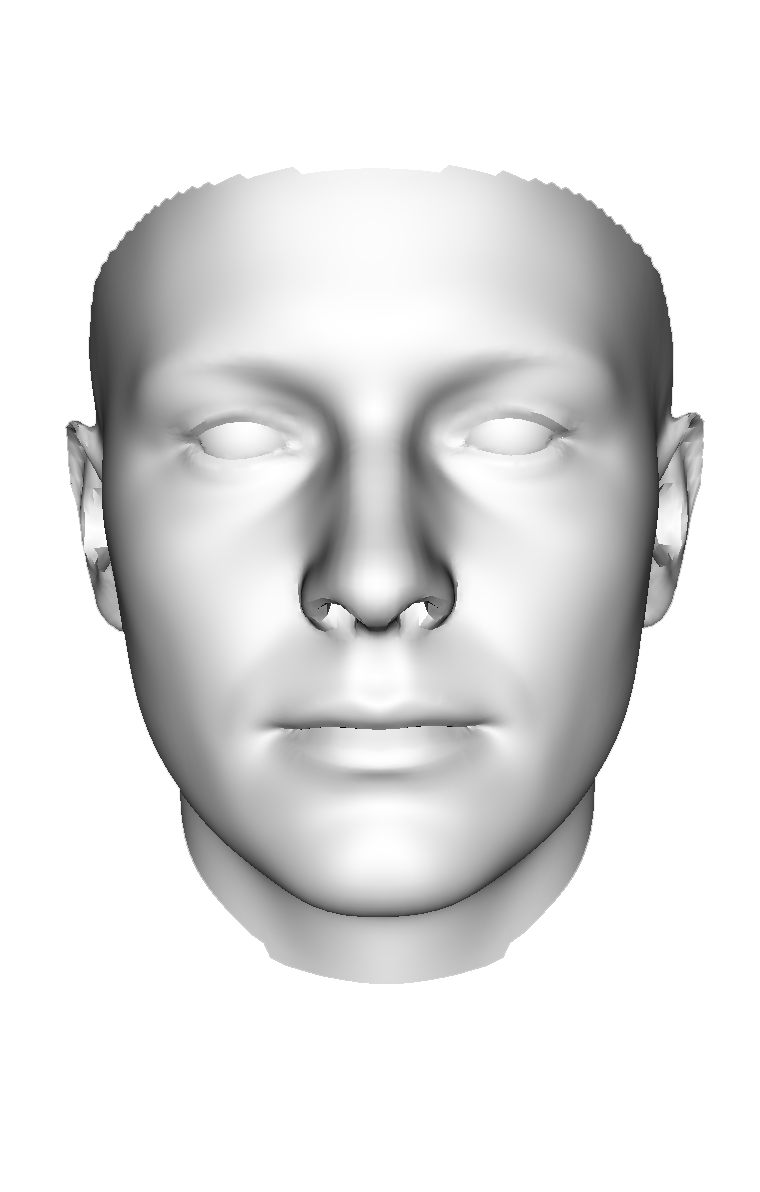
\includegraphics[width=0.2\textwidth]{img/face.png}
	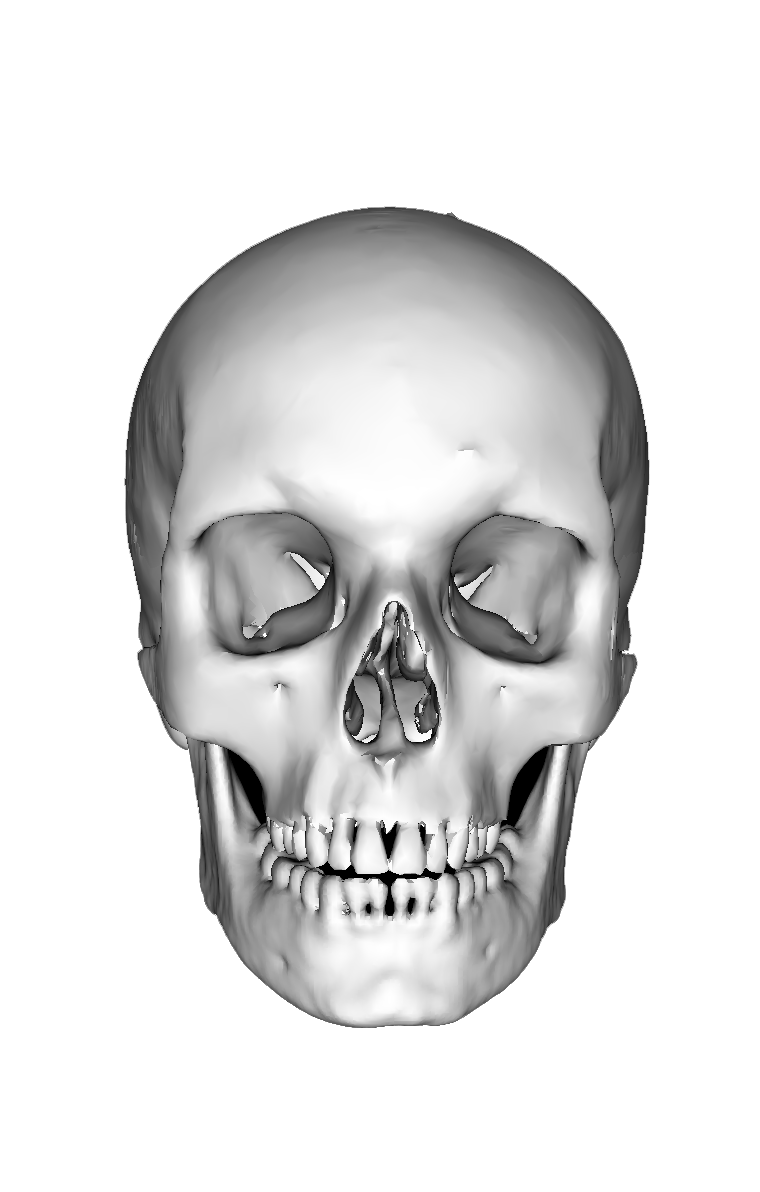
\includegraphics[width=0.2\textwidth]{img/skull.png}
	\end{center}
}
	
	%%%%%%%%%%%%%%%%%%%%%%%%%%%%%%%%%%%%%%%%%%%%%%%%%%%%%%%%%%%%%%%%%%%%%%%%%%%%%%
	\headerbox{Method}{name=method,column=0,row=0, span=2, below=overview, above=bottom}{
	%%%%%%%%%%%%%%%%%%%%%%%%%%%%%%%%%%%%%%%%%%%%%%%%%%%%%%%%%%%%%%%%%%%%%%%%%%%%%%
	\noindent Explanation of our method and citation of important papers \cite{blanz1999morphable}.

}


	%%%%%%%%%%%%%%%%%%%%%%%%%%%%%%%%%%%%%%%%%%%%%%%%%%%%%%%%%%%%%%%%%%%%%%%%%%%%%%
	\headerbox{Results}{name=resultr,column=2, span=2, below=overview}{
	%%%%%%%%%%%%%%%%%%%%%%%%%%%%%%%%%%%%%%%%%%%%%%%%%%%%%%%%%%%%%%%%%%%%%%%%%%%%%%
	\noindent Results of our work!
	\vspace{52em}
}


	%%%%%%%%%%%%%%%%%%%%%%%%%%%%%%%%%%%%%%%%%%%%%%%%%%%%%%%%%%%%%%%%%%%%%%%%%%%%%%
	\headerbox{References}{name=resultr2,column=2, span=2, below=resultr, above=bottom}{
	%%%%%%%%%%%%%%%%%%%%%%%%%%%%%%%%%%%%%%%%%%%%%%%%%%%%%%%%%%%%%%%%%%%%%%%%%%%%%%
	\AtNextBibliography{\scriptsize}
	\printbibliography[heading=none]
}
\end{poster}

\end{document}